\documentclass[a4paper,11pt]{article}
  
\usepackage{graphicx}
\usepackage{amsmath}
\usepackage{array}
\usepackage{float}
\usepackage{subfigure}
\usepackage{color}
\usepackage{listings}
\usepackage[utf8x]{inputenc}
\usepackage{hyperref}
\usepackage{rotating}

\usepackage{amsfonts}  % For \mathbb

% Read MRPT version:
\newread\file
\openin\file=../../version_prefix.txt
\read\file to\MRPTVERSION % Reads a line of the file 
\closein\file

% Title Page
\title{User guide for \texttt{libmrpt-srba}: A generic C++ framework for Relative Bundle Adjustment (RBA)}
\author{Jose-Luis Blanco Claraco \\ joseluisblancoc@gmail.com \\ \texttt{http://www.mrpt.org/} }
\date{MRPT version: \MRPTVERSION \\ Build date: \today }

\begin{document}
\maketitle

\begin{abstract}
 XXX
\end{abstract}

\newpage
\tableofcontents
\newpage

\section{Introduction}

Bundle adjustment is the name given to one solution to visual SLAM based on maximum-likelihood estimation (MLE) 
over the space of map features and camera poses. However, it is by no way limited to visual maps, since the same 
technique is also applicable to maps of pose constraints (graph-SLAM) or any other kind of feature maps not relying 
on visual information.

The framework of \textbf{Relative Bundle Adjustment (RBA)} was introduced in a series of works by Gabe Sibley and 
colleagues in \cite{sibley2009rba,sibley2009adaptive}. 

\textbf{Sparser RBA (SRBA)} is the name of the generic and extensible framework for RBA implemented in 
this C++ library, and introduced in \cite{blanco2013srba}.

\section{The \texttt{srba-slam} application}

First program


\section{Programmer's first steps}

First program

\section{Existing models}

\subsection{KF-to-KF relative poses}

XXXX XXXX 

\subsection{Relative landmark parameterizations}

XXXX XXXX 

\subsection{Observation types}

XXXX XXXX 


\section{Sensor models}

XXXX XXXX 


\section{Library inner structure}

\subsection{Directory layout}


\subsection{Data structures}


\begin{sidewaysfigure}
\centering
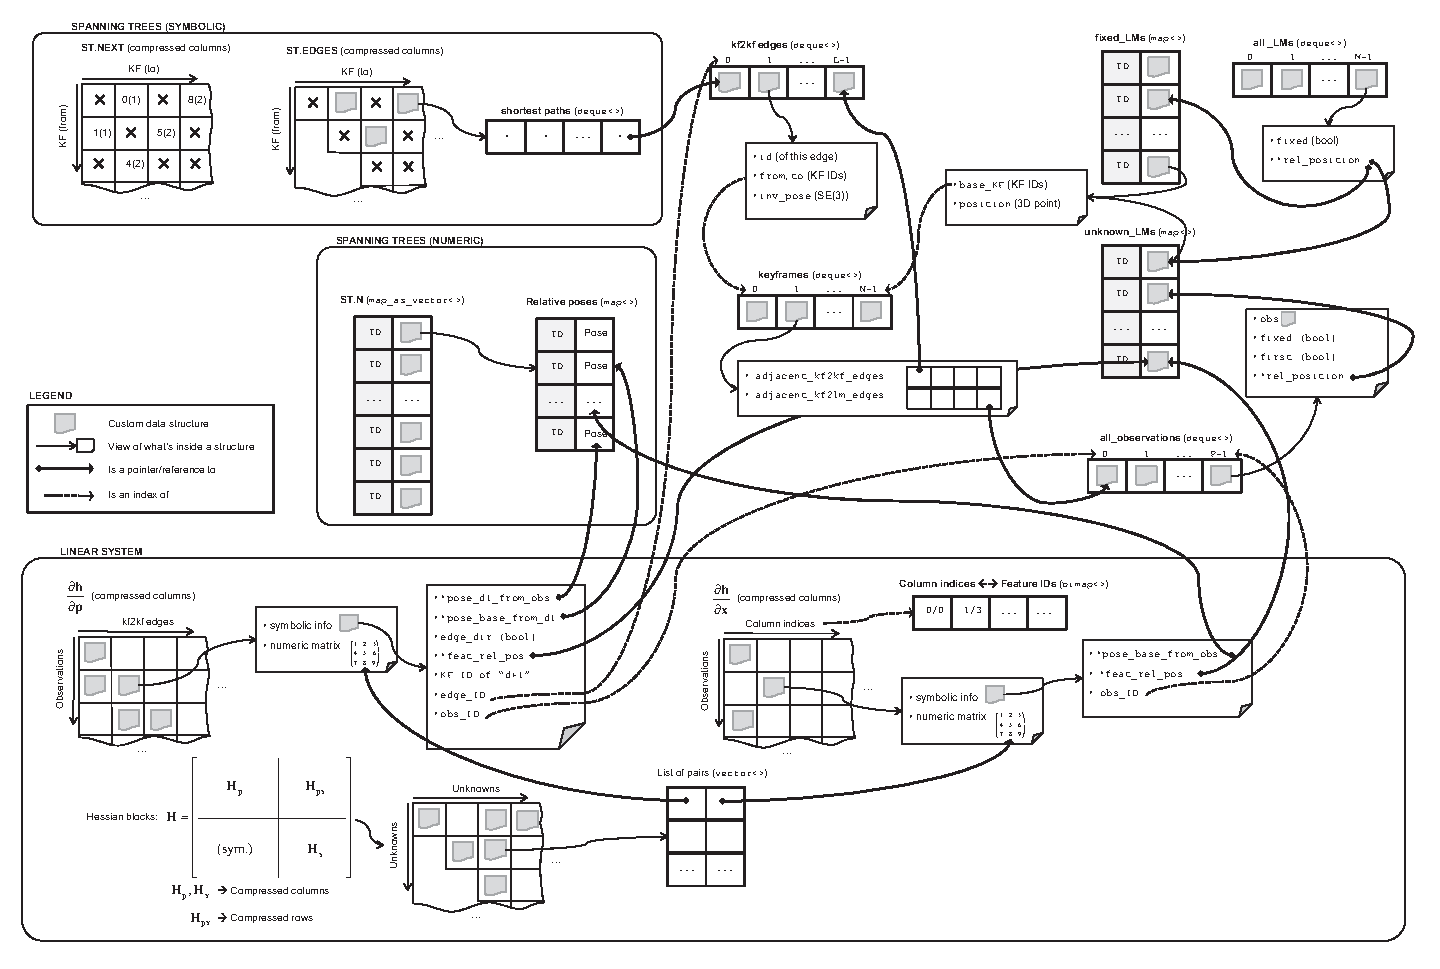
\includegraphics[width=1.0\textwidth]{imgs/srba_data_structures.eps} 
\caption{Detailed data structures. Refer to the legend for the format of structures and pointers/references.}
\label{fig:detailed.data.structures}
\end{sidewaysfigure}





%% ---------------------------------------------------------------
%%                         BIBLIOGRAPHY
%% ---------------------------------------------------------------
\newpage
\bibliographystyle{plain}
\bibliography{cites}

\end{document}

